\section{Frequent$<$ Data, Sets\-Type $>$ Class Template Reference}
\label{class_frequent}\index{Frequent@{Frequent}}
Functor representing the predicate being frequent.  


{\tt \#include $<$Frequent.hxx$>$}

Inheritance diagram for Frequent$<$ Data, Sets\-Type $>$::\begin{figure}[H]
\begin{center}
\leavevmode
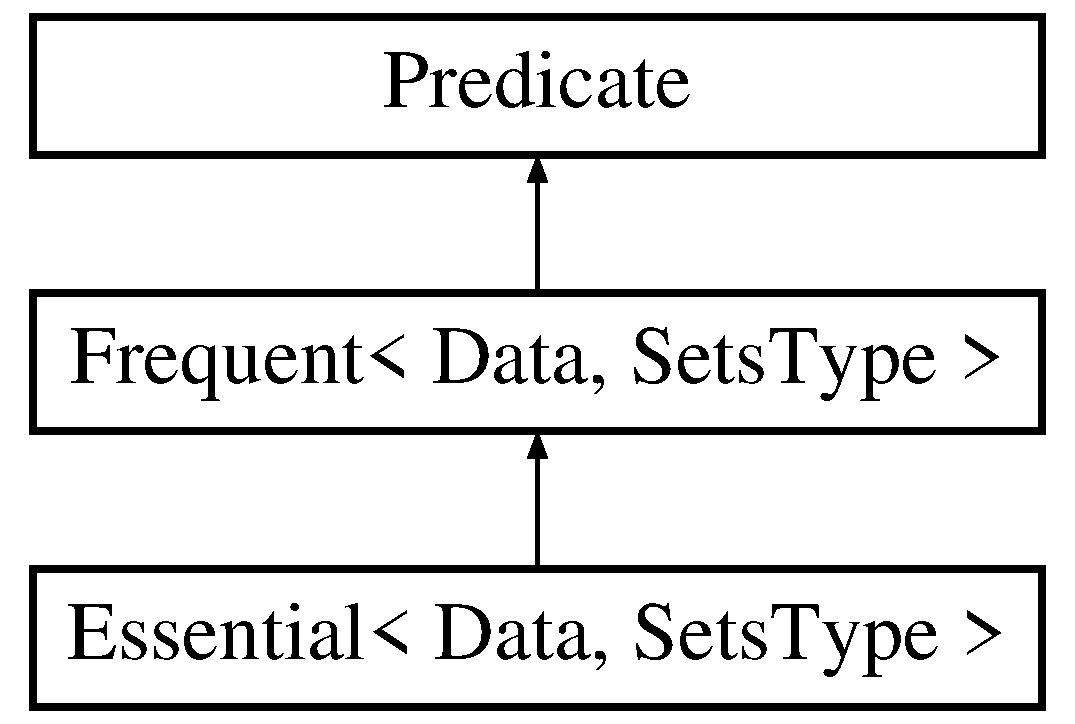
\includegraphics[height=3cm]{class_frequent}
\end{center}
\end{figure}
\subsection*{Public Member Functions}
\begin{CompactItemize}
\item 
{\bf Frequent} (Data \&indb, int in\-Minsup)
\begin{CompactList}\small\item\em Constructor. \item\end{CompactList}\item 
{\bf $\sim$Frequent} ()\label{class_frequent_c3612977fa17e8dfda09132b36a42d7f}

\begin{CompactList}\small\item\em Destructor. \item\end{CompactList}\item 
template$<$class Iterator, class Measure$>$ bool {\bf operator()} (Iterator itemset\-It, Measure \&mes\-Cand)
\begin{CompactList}\small\item\em Operator that test if an itemet is frequent or not. \item\end{CompactList}\item 
template$<$class Cand\_\-Data\-Struct, class f$>$ void {\bf pre\-Processing} (Cand\_\-Data\-Struct \&cand, f word\-To\-Set)
\begin{CompactList}\small\item\em Function used to count the support of the itemsets. \item\end{CompactList}\item 
template$<$class Cand\_\-Data\-Struct, class f$>$ void {\bf post\-Processing} (Cand\_\-Data\-Struct \&cand, f word\-To\-Set)
\begin{CompactList}\small\item\em Function used to do some post processing operations after testing the candidates generated. \item\end{CompactList}\end{CompactItemize}
\subsection*{Public Attributes}
\begin{CompactItemize}
\item 
list\-Item\-Supp {\bf list\-Item\-Support}
\begin{CompactList}\small\item\em List of all the items with their support. \item\end{CompactList}\end{CompactItemize}
\subsection*{Protected Member Functions}
\begin{CompactItemize}
\item 
template$<$class Measure, class Iterator\-Data$>$ int {\bf count} ({\bf Node}$<$ int, Measure $>$ $\ast$curr\-Node, Iterator\-Data it\-Data)
\begin{CompactList}\small\item\em Method used to count and save the support of a set of itemsets. \item\end{CompactList}\end{CompactItemize}
\subsection*{Protected Attributes}
\begin{CompactItemize}
\item 
{\bf Recode\-To\-Int}$<$ Sets\-Type $>$ {\bf recode}\label{class_frequent_3f48fefd58b3b8f45fcd4e5cc4d48931}

\begin{CompactList}\small\item\em Internal encoding of the items. \item\end{CompactList}\item 
Data $\ast$ {\bf db}\label{class_frequent_ff67dcf2a726388189b0ff9a27ef6618}

\begin{CompactList}\small\item\em The transactionnal database. \item\end{CompactList}\item 
int {\bf minsup}\label{class_frequent_23ababafb524d4f848d5e299ca2ff372}

\begin{CompactList}\small\item\em The minimum support threshold (absolute). \item\end{CompactList}\end{CompactItemize}
\subsection*{Classes}
\begin{CompactItemize}
\item 
class {\bf eq\-Item\-Supp}
\begin{CompactList}\small\item\em Functor used to find an item in the list of items/support. \item\end{CompactList}\item 
class {\bf order}
\begin{CompactList}\small\item\em Functor used to reorder a transaction. \item\end{CompactList}\item 
class {\bf reorder\-Trans}
\begin{CompactList}\small\item\em Functor that reorders a transaction and insert it in the db. \item\end{CompactList}\end{CompactItemize}


\subsection{Detailed Description}
\subsubsection*{template$<$class Data, class Sets\-Type$>$ class Frequent$<$ Data, Sets\-Type $>$}

Functor representing the predicate being frequent. 

This functor test if an itemset is frequent. This functor process the support before pruning. We suppose that the data has the same internal encoding than the candidates (ie, the first item met is recoded in \char`\"{}0\char`\"{}, the second in \char`\"{}1\char`\"{}, ...).

The methods of this predicate are specific to tries data structure ({\bf PTree}{\rm (p.\,\pageref{class_p_tree})} for the candiates and {\bf Tatree}{\rm (p.\,\pageref{class_tatree})} for the transactions). This functor cannot be used when using a transformation function (for exmaple to change the exploration of the search space).

The template parameter Data is the type of the transactional database. The template parameter Sets\-Type is the type of the items. 



\subsection{Constructor \& Destructor Documentation}
\index{Frequent@{Frequent}!Frequent@{Frequent}}
\index{Frequent@{Frequent}!Frequent@{Frequent}}
\subsubsection{\setlength{\rightskip}{0pt plus 5cm}template$<$class Data, class Sets\-Type$>$ {\bf Frequent}$<$ Data, Sets\-Type $>$::{\bf Frequent} (Data \& {\em indb}, int {\em in\-Minsup})\hspace{0.3cm}{\tt  [inline]}}\label{class_frequent_d4786ab80688426419495d0d8ff3ea47}


Constructor. 

\begin{Desc}
\item[Parameters:]
\begin{description}
\item[{\em indb}]the transactional database \item[{\em in\-Minsup}]the absolute minimum support threshold \end{description}
\end{Desc}


\subsection{Member Function Documentation}
\index{Frequent@{Frequent}!count@{count}}
\index{count@{count}!Frequent@{Frequent}}
\subsubsection{\setlength{\rightskip}{0pt plus 5cm}template$<$class Data, class Sets\-Type$>$ template$<$class Measure, class Iterator\-Data$>$ int {\bf Frequent}$<$ Data, Sets\-Type $>$::count ({\bf Node}$<$ int, Measure $>$ $\ast$ {\em curr\-Node}, Iterator\-Data {\em it\-Data})\hspace{0.3cm}{\tt  [protected]}}\label{class_frequent_50001a78dd15b91872285556ba7dfbe4}


Method used to count and save the support of a set of itemsets. 

\begin{Desc}
\item[Parameters:]
\begin{description}
\item[{\em curr\-Node}]curent node of the trie storing the itemsets \item[{\em it\-Data}]iterator on the data \end{description}
\end{Desc}
\index{Frequent@{Frequent}!operator()@{operator()}}
\index{operator()@{operator()}!Frequent@{Frequent}}
\subsubsection{\setlength{\rightskip}{0pt plus 5cm}template$<$class Data, class Sets\-Type$>$ template$<$class Iterator, class Measure$>$ bool {\bf Frequent}$<$ Data, Sets\-Type $>$::operator() (Iterator {\em itemset\-It}, Measure \& {\em mes\-Cand})\hspace{0.3cm}{\tt  [inline]}}\label{class_frequent_82e02ab1cf1749ea52e9603dc06a5d15}


Operator that test if an itemet is frequent or not. 

\begin{Desc}
\item[Parameters:]
\begin{description}
\item[{\em itemset\-It}]iterator (or pointer) on the itemset to test wrt the predicate \item[{\em mes\-Cand}]value of the support of the itemset \end{description}
\end{Desc}


Reimplemented from {\bf Predicate} {\rm (p.\,\pageref{class_predicate_6fb1a75dba2268f75738f335f403e46c})}.

Reimplemented in {\bf Essential$<$ Data, Sets\-Type $>$} {\rm (p.\,\pageref{class_essential_e6a89fa2543fe441619066b0f4f6323b})}.\index{Frequent@{Frequent}!postProcessing@{postProcessing}}
\index{postProcessing@{postProcessing}!Frequent@{Frequent}}
\subsubsection{\setlength{\rightskip}{0pt plus 5cm}template$<$class Data, class Sets\-Type$>$ template$<$class Cand\_\-Data\-Struct, class f$>$ void {\bf Frequent}$<$ Data, Sets\-Type $>$::post\-Processing (Cand\_\-Data\-Struct \& {\em cand}, f {\em word\-To\-Set})}\label{class_frequent_ff29167beb828195c34e10881abb2f74}


Function used to do some post processing operations after testing the candidates generated. 

Method used to reconstruct the db after discovery of frequent items. Prune from the transactions all the not frequent items. \begin{Desc}
\item[Parameters:]
\begin{description}
\item[{\em cand}]container of words of the language. \item[{\em word\-Toset}]functor that eventually transforms itemsets \end{description}
\end{Desc}


Reimplemented from {\bf Predicate} {\rm (p.\,\pageref{class_predicate_49f7acb334fac851a26a4d1aecc64571})}.\index{Frequent@{Frequent}!preProcessing@{preProcessing}}
\index{preProcessing@{preProcessing}!Frequent@{Frequent}}
\subsubsection{\setlength{\rightskip}{0pt plus 5cm}template$<$class Data, class Sets\-Type$>$ template$<$class Cand\_\-Data\-Struct, class f$>$ void {\bf Frequent}$<$ Data, Sets\-Type $>$::pre\-Processing (Cand\_\-Data\-Struct \& {\em cand}, f {\em word\-To\-Set})}\label{class_frequent_236bb06ebfac503436c8a25a8507b467}


Function used to count the support of the itemsets. 

Method used to count the support of itemsets. For each transaction of the db update the supports of all the itemsets in cand. \begin{Desc}
\item[Parameters:]
\begin{description}
\item[{\em cand}]container of words of the language. \item[{\em word\-Toset}]functor that eventually transforms itemsets \end{description}
\end{Desc}


Reimplemented from {\bf Predicate} {\rm (p.\,\pageref{class_predicate_8ee59d790e9b46e5e0555dbeb5b91f95})}.

\subsection{Member Data Documentation}
\index{Frequent@{Frequent}!listItemSupport@{listItemSupport}}
\index{listItemSupport@{listItemSupport}!Frequent@{Frequent}}
\subsubsection{\setlength{\rightskip}{0pt plus 5cm}template$<$class Data, class Sets\-Type$>$ list\-Item\-Supp {\bf Frequent}$<$ Data, Sets\-Type $>$::{\bf list\-Item\-Support}}\label{class_frequent_5eee2b41720ffc388e3863f54c62624f}


List of all the items with their support. 

Used to avoid support counting for items since in the initialization functor the items support is processed. Set in the initialization functor. 

The documentation for this class was generated from the following file:\begin{CompactItemize}
\item 
F:/i\-Zi/problems/frequent/Frequent.hxx\end{CompactItemize}
